\subsection{Entwurfsmuster}
Entwurfsmuster sind ein fester Bestandteil der Godot Engine.
Einige dieser Entwurfsmuster werden in der Arbeit verwendet.
Die bereits existierenden Entwurfsmuster werden zusätzlich um zwei weitere Entwurfsmuster erweitert.
Diese werden im Folgenden erläutert, allerdings wird zunächst die Grundarchitektur näher erklärt.
Komponenten oder Objekte der Architektur werden als Nodes bezeichnet.
Diese Nodes sind Teil eines Baumgraphen.
Der Wurzelknoten dieses Baumgraphen wird als Szene oder Szenengraph bezeichnet.\\

\begin{figure}[ht]
	\centering
	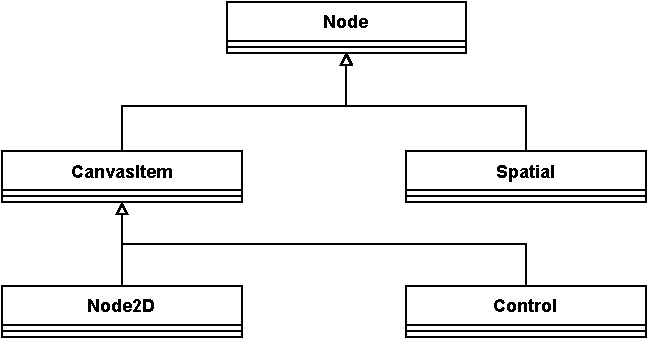
\includegraphics[width=0.8\columnwidth]{figures/node-graph.pdf}
	\caption{\label{fig:nodegraph} Node-System}
\end{figure}

\autoref{fig:nodegraph} veranschaulicht einen Ausschnitt aus dem Architekturdiagramm der Godot Engine\cite{godot-architecture}.
Spatial sind Nodes, welche eine Node im dreidimensionalen Raum abbilden.
Das bedeutet, dass ein \texttt{Transform} eines Spatial die Position, Rotation und Skalierung angibt.
Ebenfalls kann eingestellt werden, ob diese Nodes sichtbar oder nicht sichtbar sind.
Alle weiteren 3D Nodes erben von diesem Objekttyp.
Ähnliche Eigenschaften besitzen {2D Nodes}, welche von Node2D erben.
Diese befinden sich jedoch nicht im dreidimensionalen, sondern im zweidimensionalen Raum.
Die letzte Variante von Nodes sind \ac{GUI} Nodes.
Diese sind ebenfalls Teil des zweidimensionalen Raums.
Jedoch besitzen sie keinen \texttt{Transform}, sondern sind relativ zum übergeordneten Node platziert.\\

\begin{figure}[H]%
	\centering
	\subfloat[\centering Szenengraph]{{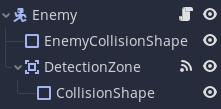
\includegraphics[width=5cm]{figures/screenshots/tree.png} }\label{fig:signal-example-a}}%
	\qquad
	\subfloat[\centering Signale]{{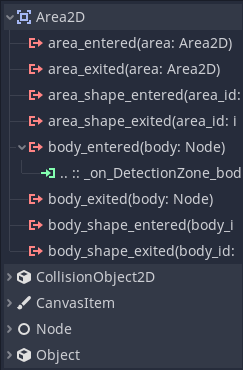
\includegraphics[width=5cm]{figures/screenshots/signals.png}
				\label{fig:signal-example-b}}}%
	\caption{Szenengraph und Signale der Area2D anhand eines Beispiels}%
	\label{fig:signal-example}%
\end{figure}

Die Godot Engine implementiert eine eigene Variante des Beobachtungsmusters\cite{godot-signals}\cite[293]{design-patterns-gof}.
Die Implementierung wird durch sogenannte Signale repräsentiert.
Jede Node besitzt Signale, welche von anderen Nodes beobachtet werden können.
\autoref{fig:signal-example} zeigt ein Beispiel, um dieses System zu verdeutlichen.
Der Szenengraph in \autoref{fig:signal-example-a} beinhaltet einen Gegner, welcher mit seiner Umgebung kollidieren kann.
Die \texttt{DetectionZone} vom Typ Area2D soll dem Gegner signalisieren, wenn ein Spieler diese Zone betritt.
Das Signal-Zeichen an der \texttt{DetectionZone}-Node symbolisiert, dass von dieser Node ein ausgehendes Signal existiert.
Dieses wird unter den verfügbaren Signalen (b) grün markiert. Ebenfalls ist zu sehen, dass neben den Signalen von Area2D noch viele weitere Signale existieren.
Parallel zu diesen, der nur für die vom Typ Area2D verfügbaren Signale, besitzt jede Node die Signale ihrer Elternklasse.
Area2D erbt von CollisionObject2D, welches von Node2D erbt. \\

Beim Auswählen eines Signals kann angegeben werden, welche Node das Signal empfängt und wie die Funktion benannt sein soll.
In diesem Fall handelt es sich um ein Signal vom Typ \texttt{body\_entered}.
Dieses wird ausgelöst, wenn eine Node vom Typ PhysicsBody2D die Area2D betritt.
Es sei angemerkt, dass mehrere Signale vom Typ \texttt{body\_entered} für eine Node existieren können.
Allerdings ist dies im angegebenen Beispiel nicht sinnvoll.
Eine Empfänger-Node muss ein Skript besitzen, weil ansonsten keine Zielfunktion angegeben werden kann.
Das Skript ist im Szenengraphen der Abbildung an der \texttt{Enemy}-Node zu erkennen.
Der Inhalt des Skripts befindet sich in \autoref{lst:signal}.\\

\definecolor{LightGray}{gray}{0.9}
\begin{listing}[H]
	\caption{Enemy.gd}
	\label{lst:signal}
	\begin{minted}[
bgcolor=LightGray,
framesep=2mm,
baselinestretch=1.2,
fontsize=\footnotesize,
linenos,
highlightlines={3}
]{gd.py:GDScriptLexer -x}
extends KinematicBody2D

func _on_DetectionZone_body_entered(body: PhysicsBody2D) -> void:
	_start_follow_player(body) # Pseudocode
\end{minted}
\end{listing}

Dieses Listing zeigt die Funktion, welche auf das Signal der Area2D reagieren soll.
Im Falle, dass ein Signal feuert, wird die Funktion aufgerufen, welche einem Spieler folgen soll.
Das Beispiel zeigt somit einen Gegner, welcher den Spieler automatisch verfolgt, sobald dieser sich in einem gewissen Radius befindet.\\

\begin{figure}[H]
	\centering
	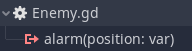
\includegraphics[width=0.4\columnwidth]{figures/screenshots/custom-signal.png}
	\caption{\label{fig:alarm} Benutzerdefiniertes Signal}
\end{figure}

Signale können ebenfalls im Code definiert und anschließend gefeuert werden.
Das vorherige Beispiel in \autoref{lst:signal} kann, wie in \autoref{lst:custom-signal} definiert, erweitert werden.
Das neue Signal erscheint dann im Editor und kann mithilfe der \texttt{connect}-Funktion oder dem Editor verbunden werden.
Der Gegner, welcher den Spieler gefunden hat, kann die globale Position als Parameter eines Signals feuern und weitere Gegner, welche auf dieses Signal hören, alarmieren.
Allerdings kann der Typ eines Signals in der ausgewählten Version der Godot Engine nicht angegeben werden.
Dies ist in Zukunft auch nicht geplant\cite{godot-signal-type}.
Aus diesem Grund ist der Typ des Signals in \autoref{fig:alarm} \texttt{var}.\\

\begin{listing}[H]
	\caption{Signale im Code}
	\label{lst:custom-signal}
	\begin{minted}
[
bgcolor=LightGray,
framesep=2mm,
baselinestretch=1.2,
fontsize=\footnotesize,
linenos,
highlightlines={3, 7},
]{gd.py:GDScriptLexer -x}
extends KinematicBody2D

signal alarm(position)

func _on_DetectionZone_body_entered(body: PhysicsBody2D) -> void:
	_start_follow_player(body) # Pseudocode
	emit_signal("alarm", body.global_position)
\end{minted}
\end{listing}

Das Problem an Signalen ist, dass diese bei einem wachsenden Projekt an vielen verschiedenen Stellen existieren und der Überblick verloren geht.
Um die Lösung für dieses Problem zu erklären, muss das von der Godot Engine implementierte Entwurfsmuster AutoLoad erläutert werden\cite{godot-autoload}.
AutoLoads sind eine Variation von Singletons\cite[S. 127]{design-patterns-gof}.
AutoLoads sind Skripte, welche beim Start der Anwendung automatisch global geladen werden.
Das bedeutet, dass sie in jeder Szene vorhanden sind.
Die Skripte können jeweils in den Projekteinstellungen konfiguriert werden.
Die Funktionsweise von AutoLoads ist nützlich, weil dadurch Code in allen anderen Skripten verfügbar ist.
Förderlich ist dies bei AutoLoads, welche zum Beispiel nur Konstanten enthalten.
Konstanten vom Typ String können verhindern, dass Tippfehler zu Fehlern führen.
Das liegt daran, dass alle Klassen, welche auf diese Konstanten zugreifen, dieselben Informationen erhalten.
Ebenfalls können auf diese Art und Weise global Minimal- oder Maximalwerte für bestimmte Variablen definiert werden.
Ein Beispiel hierfür ist die Maximalgeschwindigkeit jeder kinematischen Node, welche in einer Konstanten vom Typ Integer definiert ist.\\

\begin{listing}[H]
	\caption{Signale mit einem Eventbus}
	\label{lst:eventbus-signal}
	\begin{minted}
[
bgcolor=LightGray,
framesep=2mm,
baselinestretch=1.2,
fontsize=\footnotesize,
linenos,
highlightlines={5},
]{gd.py:GDScriptLexer -x}
extends KinematicBody2D

func _on_DetectionZone_body_entered(body: PhysicsBody2D) -> void:
	_start_follow_player(body) # Pseudocode
	EventBus.emit_signal("alarm", body.global_position)
\end{minted}
\end{listing}

Um das Problem von Signalen an unterschiedlichen Stellen im Code zu unterbinden, wurde ein Eventbus eingeführt\cite{dzone-eventbus}.
Dieses AutoLoad enthält mehrere Signale und die Skripte von Nodes können auf diese mit der \texttt{connect}-Funktion horchen.
Im Falle des erwähnten Beispiels könnte im Eventbus das Signal \texttt{alarm(position)} deklariert werden.
\autoref{lst:eventbus-signal} zeigt, wie ein Signal innerhalb einer Node über den Eventbus versendet werden kann.
Alle Nodes, welche auf dieses Event horchen, werden dann über ein aufgetretenes Signal über den Eventbus benachrichtigt.
Obwohl das Signal verwendet wird, wird die Warnung geworfen, dass das Signal nie benutzt wird.
Dies ist allerdings ein bekannter Fehler in der Spiel-Engine\cite{godot-signal-warning}.
Diese Warnung kann mithilfe eines Kommentars unterbunden werden. \\

\begin{listing}[H]
	\caption{Endlicher Automat}
	\label{lst:state-machine}
	\begin{minted}
[
bgcolor=LightGray,
framesep=2mm,
baselinestretch=1.2,
fontsize=\footnotesize,
linenos,
highlightlines={4-9, 12, 17},
]{gd.py:GDScriptLexer -x}
extends KinematicBody2D

var target: PhysicsBody2D
var state = IDLE
enum {
	IDLE,
	FOLLOW_PLAYER,
	WANDER,
}

func _physics_process(delta: float) -> void:
    _handle_state(delta)


func _on_DetectionZone_body_entered(body: PhysicsBody2D) -> void:
	target = body
	state = FOLLOW_PLAYER
	EventBus.emit_signal("alarm", body.global_position)
\end{minted}
\end{listing}

Ein weiteres Entwurfsmuster, welches in der Arbeit verwendet wird, ist das Entwurfsmuster eines endlichen Automaten\cite{gamepattern-state}.
Voraussetzung für diesen sind eine endliche Menge an Zuständen.
Im Beispiel \autoref{lst:state-machine} existieren die Zustände \texttt{IDLE}, \texttt{FOLLOW\_PLAYER} und \texttt{WANDER}.
Die Mächtigkeit dieser Menge ist drei, was bedeutet, dass sie endlich ist.
Verwendet werden solche Zustände, um Programmlogik zu separieren und Aktionen nur bestimmten Zuständen verfügbar zu machen.
Im Beispiel wechselt der Gegner zwischen den Zuständen \texttt{IDLE} und \texttt{WANDER} hin und her.
Das bedeutet, dass der Gegner entweder auf seiner Position stehen bleibt oder die Gegend erkundet.
Wenn ein Spieler die \texttt{DetectionZone} betritt, wird der Zustand auf \texttt{FOLLOW\_PLAYER} (Spieler folgen) gesetzt.
Mithilfe weiterer Funktionen kann diese Logik so umgeschrieben werden, dass der Gegner dem Spieler nur über eine bestimmte Distanz folgt und dann zum \texttt{IDLE}-Zustand zurückkehrt.\\
